%Chapter 8

\chapter{Cadenas}

Las cadenas no son como enteros, flotantes y booleanos. Una cadena es una \textbf{secuencia}, lo que significa que es una colección ordenada de otros valores. En este capítulo verás cómo acceder a los caracteres que componen una cadena y aprenderás sobre algunos de los métodos que proporcionan las cadenas.

\section{Una cadena es una secuencia}

Una cadena es una secuencia de caracteres. Puedes acceder a los caracteres uno por uno con el operador de corchetes:

\begin{lstlisting}[language=Python]
>>> fruit = 'banana'
>>> letter = fruit[1]
\end{lstlisting}

La segunda sentencia selecciona el carácter número 1 de \texttt{fruit} y lo asigna a \texttt{letter}.

La expresión entre corchetes se llama \textbf{índice}. El índice indica qué carácter de la secuencia deseas (de ahí el nombre).

Pero podrías no obtener lo que esperas:

\begin{lstlisting}[language=Python]
>>> letter
'a'
\end{lstlisting}

Para la mayoría de las personas, la primera letra de 'banana' es b, no a. Pero para los informáticos, el índice es un desplazamiento desde el inicio de la cadena, y el desplazamiento de la primera letra es cero.

\begin{lstlisting}[language=Python]
>>> letter = fruit[0]
>>> letter
'b'
\end{lstlisting}

Entonces, b es la letra 0 ("cero-ésima") de 'banana', a es la letra 1 ("uno-ésima"), y n es la letra 2 ("dos-ésima").

Como índice, puedes usar una expresión que contenga variables y operadores:

\begin{lstlisting}[language=Python]
>>> i = 1
>>> fruit[i]
'a'
>>> fruit[i+1]
'n'
\end{lstlisting}

Pero el valor del índice debe ser un entero. De lo contrario, obtendrás:

\begin{lstlisting}[language=Python]
>>> letter = fruit[1.5]
TypeError: string indices must be integers
\end{lstlisting}

\section{len}

\texttt{len} es una función incorporada que devuelve el número de caracteres en una cadena:

\begin{lstlisting}[language=Python]
>>> fruit = 'banana'
>>> len(fruit)
6
\end{lstlisting}

Para obtener la última letra de una cadena, podrías sentirte tentado a probar algo como esto:

\begin{lstlisting}[language=Python]
>>> length = len(fruit)
>>> last = fruit[length]
IndexError: string index out of range
\end{lstlisting}

La razón del \texttt{IndexError} es que no hay ninguna letra en 'banana' con el índice 6. Como comenzamos a contar desde cero, las seis letras están numeradas del 0 al 5. Para obtener el último carácter, debes restar 1 a \texttt{length}:

\begin{lstlisting}[language=Python]
>>> last = fruit[length-1]
>>> last
'a'
\end{lstlisting}

O puedes usar índices negativos, que cuentan hacia atrás desde el final de la cadena. La expresión \texttt{fruit[-1]} devuelve la última letra, \texttt{fruit[-2]} devuelve la penúltima, y así sucesivamente.

\section{Recorrido con un bucle for}

Muchos cálculos implican procesar una cadena un carácter a la vez. A menudo comienzan al principio, seleccionan cada carácter en turno, hacen algo con él y continúan hasta el final. Este patrón de procesamiento se llama \textbf{recorrido}. Una forma de escribir un recorrido es con un bucle \texttt{while}:

\begin{lstlisting}[language=Python]
index = 0
while index < len(fruit):
    letter = fruit[index]
    print(letter)
    index = index + 1
\end{lstlisting}

Este bucle recorre la cadena y muestra cada letra en una línea por sí misma. La condición del bucle es \texttt{index < len(fruit)}, por lo que cuando \texttt{index} es igual a la longitud de la cadena, la condición es falsa y el cuerpo del bucle no se ejecuta. El último carácter accedido es el que tiene el índice \texttt{len(fruit)-1}, que es el último carácter de la cadena.

Como ejercicio, escribe una función que tome una cadena como argumento y muestre las letras al revés, una por línea.

Otra forma de escribir un recorrido es con un bucle \texttt{for}:

\begin{lstlisting}[language=Python]
for letter in fruit:
    print(letter)
\end{lstlisting}

\begin{figure}[h]
        \centering
        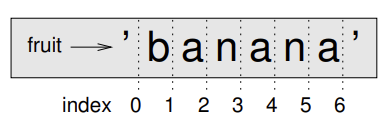
\includegraphics[width=0.5\textwidth]{./images/chapter_8_1.png}
        \caption{Slice Indices.}
        \label{fig:8_1}
        \end{figure}
Cada vez que se ejecuta el bucle, el siguiente carácter de la cadena se asigna a la variable \texttt{letter}. El bucle continúa hasta que no quedan caracteres.

El siguiente ejemplo muestra cómo usar la concatenación (suma de cadenas) y un bucle \texttt{for} para generar una serie abecedaria (es decir, en orden alfabético). En el libro \textit{Make Way for Ducklings} de Robert McCloskey, los nombres de los patitos son Jack, Kack, Lack, Mack, Nack, Quack, Pack y Quack. Este bucle imprime estos nombres en orden:

\begin{lstlisting}[language=Python]
prefixes = 'JKLMNOPQ'
suffix = 'ack'

for letter in prefixes:
    print(letter + suffix)
\end{lstlisting}

La salida es:

\begin{lstlisting}[language=Python]
Jack
Kack
Lack
Mack
Nack
Oack
Pack
Qack
\end{lstlisting}

Por supuesto, eso no es del todo correcto porque "Quack" y "Quack" están mal escritos. Como ejercicio, modifica el programa para corregir este error.

\section{Segmentos de cadena}

Un segmento de una cadena se llama \textbf{slice}. Seleccionar un slice es similar a seleccionar un carácter:

\begin{lstlisting}[language=Python]
>>> s = 'Monty Python'
>>> s[0:5]
'Monty'
>>> s[6:12]
'Python'
\end{lstlisting}

El operador \texttt{[n:m]} devuelve la parte de la cadena desde el carácter "n-ésimo" hasta el "m-ésimo", incluyendo el primero pero excluyendo el último. Este comportamiento es contraintuitivo, pero puede ayudar imaginar los índices apuntando \textit{entre} los caracteres, como en la Figura 8.1.

Si omites el primer índice (antes de los dos puntos), el slice comienza al principio de la cadena. Si omites el segundo índice, el slice llega hasta el final de la cadena:

\begin{lstlisting}[language=Python]
>>> fruit = 'banana'
>>> fruit[:3]
'ban'
>>> fruit[3:]
'ana'
\end{lstlisting}

Si el primer índice es mayor o igual que el segundo, el resultado es una cadena vacía, representada por dos comillas:

\begin{lstlisting}[language=Python]
>>> fruit = 'banana'
>>> fruit[3:3]
''
\end{lstlisting}

Una cadena vacía no contiene caracteres y tiene longitud 0, pero aparte de eso, es igual que cualquier otra cadena.

Continuando con este ejemplo, ¿qué crees que significa \texttt{fruit[:]}? Pruébalo y verás.

\section{Las cadenas son inmutables}

Es tentador usar el operador \texttt{[]} en el lado izquierdo de una asignación, con la intención de cambiar un carácter en una cadena. Por ejemplo:

\begin{lstlisting}[language=Python]
>>> greeting = 'Hello, world!'
>>> greeting[0] = 'J'
TypeError: 'str' object does not support item assignment
\end{lstlisting}

El "objeto" en este caso es la cadena y el "elemento" es el carácter que intentaste asignar. Por ahora, un objeto es lo mismo que un valor, pero refinaremos esa definición más adelante (Sección 10.10).

La razón del error es que las cadenas son \textbf{inmutables}, lo que significa que no puedes cambiar una cadena existente. Lo mejor que puedes hacer es crear una nueva cadena que sea una variación de la original:

\begin{lstlisting}[language=Python]
>>> greeting = 'Hello, world!'
>>> new_greeting = 'J' + greeting[1:]
>>> new_greeting
'Jello, world!'
\end{lstlisting}

Este ejemplo concatena una nueva primera letra con un slice de \texttt{greeting}. No tiene efecto en la cadena original.

\section{Búsqueda}

¿Qué hace la siguiente función?

\begin{lstlisting}[language=Python]
def find(word, letter):
    index = 0
    while index < len(word):
        if word[index] == letter:
            return index
        index = index + 1
    return -1
\end{lstlisting}

En cierto sentido, \texttt{find} es el inverso del operador \texttt{[]}. En lugar de tomar un índice y extraer el carácter correspondiente, toma un carácter y encuentra el índice donde aparece ese carácter. Si el carácter no se encuentra, la función devuelve -1.

Este es el primer ejemplo que vemos de una sentencia \texttt{return} dentro de un bucle. Si \texttt{word[index] == letter}, la función sale del bucle y devuelve inmediatamente.

Si el carácter no aparece en la cadena, el programa sale del bucle normalmente y devuelve -1.

Este patrón de cálculo, recorrer una secuencia y devolver cuando encontramos lo que estamos buscando, se llama \textbf{búsqueda}.

Como ejercicio, modifica \texttt{find} para que tenga un tercer parámetro, el índice en \texttt{word} donde debería comenzar a buscar.

\section{Bucles y conteo}

El siguiente programa cuenta el número de veces que aparece la letra a en una cadena:

\begin{lstlisting}[language=Python]
word = 'banana'
count = 0
for letter in word:
    if letter == 'a':
        count = count + 1
print(count)
\end{lstlisting}

Este programa demuestra otro patrón de cálculo llamado \textbf{contador}. La variable \texttt{count} se inicializa a 0 y luego se incrementa cada vez que se encuentra una a. Cuando el bucle termina, \texttt{count} contiene el resultado: el número total de a's.

Como ejercicio, encapsula este código en una función llamada \texttt{count}, y generalízala para que acepte la cadena y la letra como argumentos.

Luego reescribe la función para que, en lugar de recorrer la cadena, use la versión de tres parámetros de \texttt{find} de la sección anterior.

\section{Métodos de cadenas}

Las cadenas proporcionan métodos que realizan una variedad de operaciones útiles. Un método es similar a una función: toma argumentos y devuelve un valor, pero la sintaxis es diferente. Por ejemplo, el método \texttt{upper} toma una cadena y devuelve una nueva cadena con todas las letras en mayúsculas.

En lugar de la sintaxis de función \texttt{upper(word)}, usa la sintaxis de método \texttt{word.upper()}.

\begin{lstlisting}[language=Python]
>>> word = 'banana'
>>> new_word = word.upper()
>>> new_word
'BANANA'
\end{lstlisting}

Esta forma de notación de punto especifica el nombre del método, \texttt{upper}, y el nombre de la cadena a la que se aplica el método, \texttt{word}. Los paréntesis vacíos indican que este método no toma argumentos.

Una llamada a un método se llama \textbf{invocación}; en este caso, diríamos que estamos invocando \texttt{upper} en \texttt{word}.

Resulta que hay un método de cadena llamado \texttt{find} que es notablemente similar a la función que escribimos:

\begin{lstlisting}[language=Python]
>>> word = 'banana'
>>> index = word.find('a')
>>> index
1
\end{lstlisting}

En este ejemplo, invocamos \texttt{find} en \texttt{word} y pasamos la letra que estamos buscando como parámetro.

En realidad, el método \texttt{find} es más general que nuestra función; puede encontrar subcadenas, no solo caracteres:

\begin{lstlisting}[language=Python]
>>> word.find('na')
2
\end{lstlisting}

Por defecto, \texttt{find} comienza al principio de la cadena, pero puede tomar un segundo argumento, el índice donde debería comenzar a buscar:

\begin{lstlisting}[language=Python]
>>> word.find('na', 3)
4
\end{lstlisting}

Este es un ejemplo de un \textbf{argumento opcional}; \texttt{find} también puede tomar un tercer argumento, el índice donde debería detenerse:

\begin{lstlisting}[language=Python]
>>> name = 'bob'
>>> name.find('b', 1, 2)
-1
\end{lstlisting}

Esta búsqueda falla porque b no aparece en el rango de índices de 1 a 2, sin incluir 2. Buscar hasta, pero sin incluir, el segundo índice hace que \texttt{find} sea consistente con el operador de slice.

\section{El operador in}

La palabra \texttt{in} es un operador booleano que toma dos cadenas y devuelve \texttt{True} si la primera aparece como subcadena en la segunda:

\begin{lstlisting}[language=Python]
>>> 'a' in 'banana'
True
>>> 'seed' in 'banana'
False
\end{lstlisting}

Por ejemplo, la siguiente función imprime todas las letras de \texttt{word1} que también aparecen en \texttt{word2}:

\begin{lstlisting}[language=Python]
def in_both(word1, word2):
    for letter in word1:
        if letter in word2:
            print(letter)
\end{lstlisting}

Con nombres de variables bien elegidos, Python a veces se lee como inglés. Podrías leer este bucle como: "para (cada) letra en (la primera) palabra, si (la) letra (aparece) en (la segunda) palabra, imprime (la) letra."

Esto es lo que obtienes si comparas manzanas y naranjas:

\begin{lstlisting}[language=Python]
>>> in_both('apples', 'oranges')
a
e
s
\end{lstlisting}

\section{Comparación de cadenas}

Los operadores relacionales funcionan con cadenas. Para ver si dos cadenas son iguales:

\begin{lstlisting}[language=Python]
if word == 'banana':
    print('All right, bananas.')
\end{lstlisting}

Otras operaciones relacionales son útiles para poner palabras en orden alfabético:

\begin{lstlisting}[language=Python]
if word < 'banana':
    print('Your word, ' + word + ', comes before banana.')
elif word > 'banana':
    print('Your word, ' + word + ', comes after banana.')
else:
    print('All right, bananas.')
\end{lstlisting}

Python no maneja las letras mayúsculas y minúsculas de la misma manera que las personas. Todas las letras mayúsculas vienen antes de todas las letras minúsculas, por lo que:

\begin{lstlisting}[language=Python]
Your word, Pineapple, comes before banana.
\end{lstlisting}

Una forma común de abordar este problema es convertir las cadenas a un formato estándar, como todas minúsculas, antes de realizar la comparación. Tenlo en cuenta en caso de que tengas que defenderte de un hombre armado con una Piña.

\section{Depuración}

Cuando usas índices para recorrer los valores en una secuencia, es complicado acertar con el inicio y el final del recorrido. Aquí hay una función que se supone que compara dos palabras y devuelve \texttt{True} si una de las palabras es el reverso de la otra, pero contiene dos errores:

\begin{lstlisting}[language=Python]
def is_reverse(word1, word2):
    if len(word1) != len(word2):
        return False
    i = 0
    j = len(word2)
    while j > 0:
        if word1[i] != word2[j]:
            return False
        i = i+1
        j = j-1
    return True
\end{lstlisting}

La primera sentencia \texttt{if} verifica si las palabras tienen la misma longitud. Si no, podemos devolver \texttt{False} inmediatamente. De lo contrario, para el resto de la función, podemos asumir que las palabras tienen la misma longitud. Este es un ejemplo del patrón guardián de la Sección 6.8.

\texttt{i} y \texttt{j} son índices: \texttt{i} recorre \texttt{word1} hacia adelante mientras que \texttt{j} recorre \texttt{word2} hacia atrás. Si encontramos dos letras que no coinciden, podemos devolver \texttt{False} inmediatamente. Si llegamos al final del bucle y todas las letras coinciden, devolvemos \texttt{True}.

Si probamos esta función con las palabras "pots" y "stop", esperamos que devuelva \texttt{True}, pero obtenemos un \texttt{IndexError}:

\begin{lstlisting}[language=Python]
>>> is_reverse('pots', 'stop')
...
File "reverse.py", line 15, in is_reverse
    if word1[i] != word2[j]:
IndexError: string index out of range
\end{lstlisting}

Para depurar este tipo de error, mi primer movimiento es imprimir los valores de los índices inmediatamente antes de la línea donde aparece el error.

\begin{lstlisting}[language=Python]
while j > 0:
    print(i, j) # print here
    if word1[i] != word2[j]:
        return False
    i = i+1
    j = j-1
\end{lstlisting}

Ahora cuando ejecuto el programa de nuevo, obtengo más información:

\begin{lstlisting}[language=Python]
>>> is_reverse('pots', 'stop')
0 4
...
IndexError: string index out of range
\end{lstlisting}

La primera vez que se ejecuta el bucle, el valor de \texttt{j} es 4, que está fuera de rango para la cadena 'pots'. El índice del último carácter es 3, por lo que el valor inicial para \texttt{j} debería ser \texttt{len(word2)-1}.

Si arreglo ese error y ejecuto el programa de nuevo, obtengo:

\begin{lstlisting}[language=Python]
>>> is_reverse('pots', 'stop')
0 3
1 2
2 1
True
\end{lstlisting}

Esta vez obtenemos la respuesta correcta, pero parece que el bucle solo se ejecutó tres veces, lo cual es sospechoso. Para tener una mejor idea de lo que está sucediendo, es útil dibujar un diagrama de estado. Durante la primera iteración, el marco para \texttt{is\_reverse} se muestra en la Figura 8.2.

Tomé algunas libertades al organizar las variables en el marco y agregué líneas punteadas para mostrar que los valores de \texttt{i} y \texttt{j} indican caracteres en \texttt{word1} y \texttt{word2}.

A partir de este diagrama, ejecuta el programa en papel, cambiando los valores de \texttt{i} y \texttt{j} durante cada iteración. Encuentra y corrige el segundo error en esta función.

\begin{figure}[h]
        \centering
        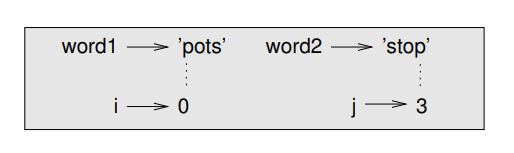
\includegraphics[width=0.5\textwidth]{./images/chapter_8_2.png}
        \caption{Turtle Pies.}
        \label{fig:8_2}
        \end{figure}

\section{Glosario}

\begin{description}
\item[objeto:] Algo a lo que una variable puede referirse. Por ahora, puedes usar "objeto" y "valor" indistintamente.
\item[secuencia:] Una colección ordenada de valores donde cada valor se identifica por un índice entero.
\item[elemento:] Uno de los valores en una secuencia.
\item[índice:] Un valor entero utilizado para seleccionar un elemento en una secuencia, como un carácter en una cadena. En Python, los índices comienzan desde 0.
\item[slice:] Una parte de una cadena especificada por un rango de índices.
\item[cadena vacía:] Una cadena sin caracteres y de longitud 0, representada por dos comillas.
\item[inmutable:] La propiedad de una secuencia cuyos elementos no pueden cambiarse.
\item[recorrer:] Iterar a través de los elementos en una secuencia, realizando una operación similar en cada uno.
\item[búsqueda:] Un patrón de recorrido que se detiene cuando encuentra lo que está buscando.
\item[contador:] Una variable utilizada para contar algo, generalmente inicializada a cero y luego incrementada.
\item[invocación:] Una sentencia que llama a un método.
\item[argumento opcional:] Un argumento de función o método que no es obligatorio.
\end{description}

\section{Ejercicios}

\textbf{Ejercicio 8.1.} Lee la documentación de los métodos de cadena en \url{http://docs.python.org/3/library/stdtypes.html#string-methods}. Es posible que desees experimentar con algunos de ellos para asegurarte de que entiendes cómo funcionan. \texttt{strip} y \texttt{replace} son particularmente útiles.

La documentación utiliza una sintaxis que podría ser confusa. Por ejemplo, en \texttt{find(sub[, start[, end]])}, los corchetes indican argumentos opcionales. Entonces \texttt{sub} es obligatorio, pero \texttt{start} es opcional, y si incluyes \texttt{start}, entonces \texttt{end} es opcional.

\textbf{Ejercicio 8.2.} Hay un método de cadena llamado \texttt{count} que es similar a la función en la Sección 8.7. Lee la documentación de este método y escribe una invocación que cuente el número de a's en 'banana'.

\textbf{Ejercicio 8.3.} Un slice de cadena puede tomar un tercer índice que especifica el "tamaño del paso"; es decir, el número de espacios entre caracteres sucesivos. Un tamaño de paso de 2 significa cada segundo carácter; 3 significa cada tercero, etc.

\begin{lstlisting}[language=Python]
>>> fruit = 'banana'
>>> fruit[0:5:2]
'bmn'
\end{lstlisting}

Un tamaño de paso de -1 recorre la palabra hacia atrás, por lo que el slice \texttt{[::-1]} genera una cadena invertida.

Usa este modismo para escribir una versión en una sola línea de \texttt{is\_palindrome} del Ejercicio 6.3.

\textbf{Ejercicio 8.4.} Las siguientes funciones están destinadas a verificar si una cadena contiene letras minúsculas, pero al menos algunas de ellas son incorrectas. Para cada función, describe qué hace realmente la función (asumiendo que el parámetro es una cadena).

\begin{lstlisting}[language=Python]
def any_lowercase1(s):
    for c in s:
        if c.islower():
            return True
        else:
            return False

def any_lowercase2(s):
    for c in s:
        if 'c'.islower():
            return 'True'
        else:
            return 'False'

def any_lowercase3(s):
    for c in s:
        flag = c.islower()
    return flag

def any_lowercase4(s):
    flag = False
    for c in s:
        flag = flag or c.islower()
    return flag

def any_lowercase5(s):
    for c in s:
        if not c.islower():
            return False
    return True
\end{lstlisting}

\textbf{Ejercicio 8.5.} Un cifrado César es una forma débil de encriptación que implica ``rotar'' cada letra por un número fijo de lugares. Rotar una letra significa desplazarla a través del alfabeto, volviendo al principio si es necesario, de modo que \texttt{'A'} rotada por 3 es \texttt{'D'} y \texttt{'Z'} rotada por 1 es \texttt{'A'}.

Para rotar una palabra, rota cada letra por la misma cantidad. Por ejemplo, \texttt{"cheer"} rotada por 7 es \texttt{"jolly"} y \texttt{"melon"} rotada por -10 es \texttt{"cubed"}. En la película \textit{2001: Una odisea del espacio}, la computadora de la nave se llama \texttt{HAL}, que es \texttt{IBM} rotada por -1.

Escribe una función llamada \texttt{rotate\_word} que tome una cadena y un entero como parámetros, y devuelva una nueva cadena que contenga las letras de la cadena original rotadas por la cantidad dada.

Es posible que desees usar la función incorporada \texttt{ord}, que convierte un carácter en un código numérico, y \texttt{chr}, que convierte códigos numéricos en caracteres. Las letras del alfabeto están codificadas en orden alfabético, por lo que, por ejemplo:

\begin{lstlisting}[language=Python]
>>> ord('c') - ord('a')
2
\end{lstlisting}

Porque 'c' es la segunda letra del alfabeto. Pero ten cuidado: los códigos numéricos para las letras mayúsculas son diferentes.

Los chistes potencialmente ofensivos en Internet a veces están codificados en ROT13, que es un cifrado César con rotación 13. Si no te ofendes fácilmente, busca y decodifica algunos de ellos. Solución: \url{https://thinkpython.com/code/rotate.py}.